\documentclass[handout]{beamer}
\usetheme{Marburg}
\useoutertheme{infolines}
\newcommand{\answers}{1}

\usepackage{amsmath}
\usepackage{caption}
\usepackage{color}
\usepackage{enumerate}
\usepackage{listings}
\usepackage{hyperref}
\usepackage{mathrsfs}
\usepackage{natbib}
\usepackage{url}

\providecommand{\all}{\ \forall \ }
\providecommand{\bs}{\backslash}
\providecommand{\e}{\varepsilon}
\providecommand{\E}{\ \exists \ }
\providecommand{\lm}[2]{\lim_{#1 \rightarrow #2}}
\providecommand{\m}[1]{\mathbb{#1}}
\providecommand{\nv}{{}^{-1}}
\providecommand{\ov}[1]{\overline{#1}}
\providecommand{\p}{\newpage}
\providecommand{\q}{$\quad$ \newline}
\providecommand{\rt}{\rightarrow}
\providecommand{\Rt}{\Rightarrow}
\providecommand{\vc}[1]{\boldsymbol{#1}}
\providecommand{\wh}[1]{\widehat{#1}}

\hypersetup{colorlinks,linkcolor=,urlcolor=blue}
\numberwithin{equation}{section}

\definecolor{dkgreen}{rgb}{0,0.6,0}
\definecolor{gray}{rgb}{0.5,0.5,0.5}
\definecolor{mauve}{rgb}{0.58,0,0.82}

\lstset{ 
  language=C,                % the language of the code
  basicstyle= \tiny,           % the size of the fonts that are used for the code
  numbers=left,
  numberfirstline=true,
  numbersep=5pt,                  % how far the line-numbers are from the code
  backgroundcolor=\color{white},      % choose the background color. You must add \usepackage{color}
  showspaces=false,               % show spaces adding particular underscores
  showstringspaces=false,         % underline spaces within strings
  showtabs=false,                 % show tabs within strings adding particular underscores
  frame=lrb,                   % adds a frame around the code
  rulecolor=\color{black},        % if not set, the frame-color may be changed on line-breaks within not-black text 
  tabsize=2,                      % sets default tabsize to 2 spaces
  captionpos=t,                   % sets the caption-position 
  breaklines=true,                % sets automatic line breaking
  breakatwhitespace=false,        % sets if automatic breaks should only happen at whitespace
  %title=\lstname,                   % show the filename of files included with \lstinputlisting;
  keywordstyle=\color{blue},          % keyword style
  commentstyle=\color{gray},       % comment style
  stringstyle=\color{dkgreen},         % string literal style
  escapeinside={\%*}{*)},            % if you want to add LaTeX within your code
  morekeywords={*, ...},               % if you want to add more keywords to the set
  xleftmargin=0.053in, % left horizontal offset of caption box
  xrightmargin=-.03in % right horizontal offset of caption box
}

%\DeclareCaptionFont{white}{\color{white}}
%\DeclareCaptionFormat{listing}{\parbox{\textwidth}{\colorbox{gray}{\parbox{\textwidth}{#1#2#3}}\vskip-0.05in}}
%\captionsetup[lstlisting]{format = listing, labelfont = white, textfont = white}
%For caption-free listings, comment out the 3 lines above and uncomment the 2 lines below.
 \captionsetup{labelformat = empty, labelsep = none}
 \lstset{frame = single}

\title{The Thrust library}
\author{Will Landau}
\date{November 11, 2013}
\institute{Iowa State University}

\begin{document}

\begin{frame}
\titlepage
 \end{frame}
 
 \begin{frame}
\frametitle{Outline}
\tableofcontents
\end{frame}
 
 \AtBeginSection[]
{
   \begin{frame}
       \frametitle{Outline}
       \tableofcontents[currentsection]
   \end{frame}
}

\section{Getting started}

\begin{frame}
\frametitle{Background}
\begin{itemize}
\item Thrust is the CUDA analog of the Standard Template Library (STL) of C++. It comes with any installation of CUDA 4.2 and above and features:

\begin{itemize}
\pause \item Dynamic data structures
\pause \item An encapsulation of GPU/CPU communication, memory management, and other low-level tasks.
\pause \item High-performance GPU-accelerated algorithms such as sorting and reduction
\end{itemize}

\pause \item Brief history:
\begin{itemize}
\pause \item Emerged from Komrade (deprecated) in 2009
\pause \item Maintained primarily by Jared Hoberock and Nathan Bell of NVIDIA.
\end{itemize}
\end{itemize}
\end{frame}


\begin{frame}[fragile]
\frametitle{{\tt vector1.cu}}
\begin{lstlisting}[name=v1]
#include <thrust/host_vector.h> 
#include <thrust/device_vector.h>
#include <iostream>

int main(void){

  // H has storage for 4 integers
  thrust::host_vector<int> H(4);

  // initialize individual elements
  H[0] = 14;
  H[1] = 20;
  H[2] = 38;
  H[3] = 46;

  // H.size() returns the size of vector H
  std::cout << "H has size " << H.size() << std::endl;

  // print contents of H
  for(int i = 0; i < H.size(); i++)
    std::cout << "H[" << i << "] = " << H[i] << std::endl;

  // resize H
  H.resize(2);
  std::cout << "H now has size " << H.size() << std::endl;

  // Copy host_vector H to device_vector D
  thrust::device_vector<int> D = H;
\end{lstlisting}
\end{frame}

\begin{frame}[fragile]
\frametitle{{\tt vector1.cu}}
\begin{lstlisting}[name=v1]
  // elements of D can be modified
  D[0] = 99; 
  D[1] = 88;
  
  // print contents of D
  for(int i = 0; i < D.size(); i++)
    std::cout << "D[" << i << "] = " << D[i] << std::endl;

  // H and D are automatically deleted when the function returns
  return 0;
}
\end{lstlisting}

\pause \begin{lstlisting}
> nvcc vector1.cu -o vector1
> ./vector1
H has size 4
H[0] = 14
H[1] = 20
H[2] = 38
H[3] = 46
H now has size 2
D[0] = 99
D[1] = 88
\end{lstlisting}
\end{frame}


\begin{frame}
\frametitle{Notes}
\begin{itemize}
\item Thrust takes care of {\tt malloc(), cudaMalloc(), free(), and cudaFree()} for you without sacrificing performance.
\pause \item The ``=" operator does a {cudaMemcpy()} if one vector is on the host and one is on the device.
\pause \item {\tt thrust::} and {\tt std::} clarify the \emph{namespace} of the function after the double colon. For example, we need to distinguish between {\tt thrust::copy()} and {\tt std::copy()}. 
\pause \item The ``$<<$" operator sends a value to an output stream, the C++ alternative to {\tt printf()}. 
\end{itemize}
\end{frame}

\begin{frame}[fragile]
\frametitle{{\tt vector2.cu}}
\begin{lstlisting}[name=v2]
#include <thrust/host_vector.h> 
#include <thrust/device_vector.h>
#include <thrust/copy.h>
#include <thrust/fill.h> 
#include <thrust/sequence.h>
#include <iostream>

int main(void){
  // initialize all ten integers of a device_vector to 1
  thrust::device_vector <int> D(10, 1);

  // set the first seven elements of a vector to 9
  thrust::fill(D.begin(), D.begin() + 7, 9);

  // initialize a host_vector with the first five elements of D
  thrust::host_vector<int> H(D.begin(), D.begin() + 5);

  // set the elements of H to 0, 1, 2, 3, ...
  thrust::sequence(H.begin(), H.end());

  // copy all of H back to the beginning of D
  thrust::copy(H.begin(), H.end(), D.begin());

  // print D
  for(int i = 0; i < D.size(); i++)
    std::cout << "D[" << i << "] = " << D[i] << std::endl;

  return 0; 
}
\end{lstlisting}
\end{frame}


\begin{frame}[fragile]
\frametitle{{\tt vector2.cu}}
\begin{lstlisting}[name=v2]
[landau@impact1 vector2]$ make
nvcc vector2.cu -o vector2
[landau@impact1 vector2]$ ./vector2
D[0] = 0
D[1] = 1
D[2] = 2
D[3] = 3
D[4] = 4
D[5] = 9
D[6] = 9
D[7] = 1
D[8] = 1
D[9] = 1
[landau@impact1 vector2]$ 
\end{lstlisting}
\end{frame}

\begin{frame}
\frametitle{Assignment}
\begin{itemize}
\item  {\tt thrust::copy()} copies a section of one vector into a section of another.
\pause \item {\tt thrust::fill()} sets a range of elements to some fixed value. 
\pause \item {\tt thrust::sequence()} assigns equally-spaced values to a section of a vector.
\end{itemize}
\end{frame}

\begin{frame}
\frametitle{The vector template classes}
\begin{itemize}
\item Declaring vectors:
\begin{itemize}
\pause \item {\tt thrust::device\_vector<T> D;} creates a vector {\tt D} with entries of data type {\tt T} on the device.
\pause \item The analogous declaration for host vectors is {\tt thrust:: host\_vector<T> H;}.
\end{itemize}
\pause \item An object {\tt D} of the vector template class includes the following features:
\begin{itemize}
\pause \item A dynamic linear array of elements of type {\tt T}.
\pause \item Two \emph{iterators}:
\begin{itemize}
\pause \item {\tt D.begin()}
\item {\tt D.end()}
\end{itemize}
\end{itemize}
\end{itemize}
\end{frame}



\section{Iterators}

\begin{frame}[fragile]
\frametitle{Basic iterators}
\begin{itemize}
\item An iterator is a pointer with a C++ wrapper around it. The wrapper contains additional information, such as whether the vector is stored on the host or the device.
\end{itemize}

\pause \begin{lstlisting}
// allocate device vector
thrust::device_vector<int> d_vec(4);

d_vec.begin(); // returns iterator at first element of d_vec
d_vec.end(); // returns iterator one past the last element of d_vec 

// [begin, end) pair defines a sequence of 4 elements
\end{lstlisting}


\begin{center}
\setkeys{Gin}{width=.4\textwidth} 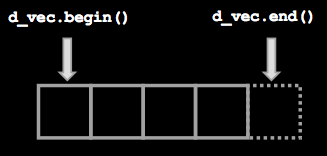
\includegraphics{../../fig/iter.png}
\end{center}
\end{frame}

\begin{frame}[fragile]
\frametitle{Iterators act like pointers.}

\begin{lstlisting}
// allocate device vector
thrust::device_vector<int> d_vec(4);

thrust::device_vector<int>::iterator begin = d_vec.begin();
thrust::device_vector<int>::iterator end = d_vec.end();

int length = end - begin; // compute the length of the vector

end = d_vec.begin() + 3; // define a sequence of 3 elements
\end{lstlisting}

\begin{center}
\setkeys{Gin}{width=.4\textwidth} 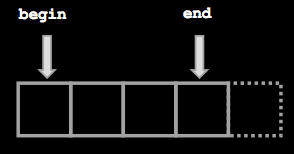
\includegraphics{../../fig/iter2.png}
\end{center}
\end{frame}

\begin{frame}[fragile]
\frametitle{Using iterators}
\begin{lstlisting}
// allocate device vector
thrust::device_vector<int> d_vec(4);

thrust::device_vector<int>::iterator begin = d_vec.begin();

*begin = 13; // same as d_vec[0] = 13; 
int temp = *begin; // same as temp = d_vec[0];

begin++; // advance iterator one position 

*begin = 25; // same as d_vec[1] = 25;
\end{lstlisting}
\end{frame}

\begin{frame}[fragile]
\frametitle{Wrap pointers to make iterators.}
\begin{lstlisting}
int N = 10;

// raw pointer to device memory
int * raw_ptr;
cudaMalloc((void **) &raw_ptr, N * sizeof(int));

// wrap raw pointer with a device_ptr
thrust::device_ptr<int> dev_iter(raw_ptr); // dev_iter is now an iterator pointing to device memory
thrust::fill(dev_iter, dev_iter + N, (int) 0); // access device memory through device_ptr

dev_iter[0] = 1;

// free memory
cudaFree(raw_ptr);
\end{lstlisting}
\end{frame}

\begin{frame}[fragile]
\frametitle{Unwrap iterators to extract pointers.}
\begin{lstlisting}
// allocate device vector
thrust::device_vector<int> d_vec(4);

// obtain raw pointer to device vector�s memory
int * ptr = thrust::raw_pointer_cast(&d_vec[0]); // use ptr in a CUDA C kernel
my_kernel<<<N/256, 256>>>(N, ptr);

// Note: ptr cannot be dereferenced on the host!
\end{lstlisting}
\end{frame}



\begin{frame}[fragile]
\frametitle{\tt constant\_iterator}
\begin{itemize}
\item A {\tt constant\_iterator} is a pointer with some constant value associated with it. 
\end{itemize}

\pause \begin{lstlisting}
#include <thrust/iterator/constant_iterator.h>
...
// create iterators
thrust::constant_iterator <int> first(10); 
thrust::constant_iterator <int> last = first + 3;

first[0]; // returns 10
first[1]; // returns 10 
first[100]; // returns 10

// sum of [first , last)
thrust::reduce(first, last); // returns 30 (i.e. 3 * 10)
\end{lstlisting}
\end{frame}


\begin{frame}[fragile]
\frametitle{\tt counting\_iterator}

\begin{itemize}
\item A {\tt counting\_iterator} is a pointer with the value {\tt some\_constant + offset} associated with it. 
\end{itemize}

\pause \begin{lstlisting}
#include <thrust/iterator/counting_iterator.h> 
...

// create iterators
thrust::counting_iterator <int> first(10);
thrust::counting_iterator <int> last = first + 3;

first[0]; // returns 10 
first[1]; // returns 11
first[100]; // returns 110

// sum of [first , last)
thrust::reduce(first, last); // returns 33 (i.e. 10 + 11 + 12)
\end{lstlisting}
\end{frame}


\begin{frame}[fragile]
\frametitle{\tt transform\_iterator}
\begin{itemize}
\item A {\tt transform\_iterator} is a pointer with the value {\tt some\_function(vector\_entry)} associated with it.
\end{itemize}

\pause \begin{lstlisting}
#include <thrust/iterator/transform_iterator.h> 
...
thrust::device_vector <int> vec(3); 
vec[0] = 10; 
vec[1] = 20; 
vec[2] = 30;

// create iterator 
thrust::transform_iterator <int> first = 
  thrust::make_transform_iterator(vec.begin(), negate<int>());

thrust::transform_iterator <int> last = 
  thrust::make_transform_iterator(vec.end(), negate<int>());

first[0] // returns -10 
first[1] // returns -20
first[2] // returns -30

thrust::reduce(first, last); // returns -60 (i.e. -10 + -20 + -30)

//same thing:
thrust::reduce(
  thrust::make_transform_iterator(
    vec.begin(), negate<int>()),
  thrust::make_transform_iterator(
    vec.end(), negate<int>()));
\end{lstlisting}
\end{frame}

\begin{frame}[fragile]
\frametitle{\tt permutation\_iterator}
\begin{itemize}
\item A {\tt permutation\_iterator} is a pointer associated with a permuted vector. 
\end{itemize}

\pause \begin{lstlisting}[name=pi]
#include <thrust/iterator/permutation_iterator.h>
...
thrust::device_vector <int> map(4); 
map[0] = 3;
map[1] = 1; 
map[2] = 0;
map[3] = 5;

thrust::device_vector <int> source(6);
source[0] = 10; 
source[1] = 20;
source[2] = 30; 
source[3] = 40;
source[4] = 50; 
source[5] = 60;

typedef thrust::device_vector<int>::iterator indexIter;

thrust::permutation_iterator<indexIter, indexIter> pbegin = 
  thrust::make_permutation_iterator(
    source.begin(), map.begin());

thrust::permutation_iterator<indexIter, indexIter> pend = 
  thrust::make_permutation_iterator(
    source.end(), map.end());
\end{lstlisting}
\end{frame}


\begin{frame}[fragile]
\frametitle{\tt permutation\_iterator}
\begin{lstlisting}[name=pi]
int p0 = pbegin[0]; // source[map[0]] = 40
int p1 = pbegin[1]; // source[map[1]] = 20

int sum = thrust::reduce(pbegin, pend);
  
/* sum = 
 * source[map[0]] + source[map[1]] + source[map[2]] + source[map[3]] =
 * source[3] + source[1] + source[0] + source[5] =
 * 40 + 20 + 10 + 60 =
 * 130 */
\end{lstlisting}
\end{frame}

\begin{frame}[fragile]
\frametitle{\tt zip\_iterator}

\begin{itemize}
\item A {\tt zip\_iterator} is a pointer associated with a vector of tuples.
\end{itemize}

\pause \begin{lstlisting}[name=zip]
#include <thrust/device_vector.h>
#include <thrust/tuple.h>
#include <thrust/iterator/zip_iterator.h>
#include <iostream>

#include <thrust/iterator/zip_iterator.h>

int main(){
  thrust::device_vector<int> int_v(3);
  int_v[0] = 0; int_v[1] = 1; int_v[2] = 2;

  thrust::device_vector<float> float_v(3);
  float_v[0] = 0.0; float_v[1] = 1.0; float_v[2] = 2.0;

  thrust::device_vector<char> char_v(3);
  char_v[0] = 'a'; char_v[1] = 'b'; char_v[2] = 'c';

  // typedef these iterators for shorthand
  typedef thrust::device_vector<int>::iterator   IntIterator;
  typedef thrust::device_vector<float>::iterator FloatIterator;
  typedef thrust::device_vector<char>::iterator  CharIterator;
\end{lstlisting}
\end{frame}

\begin{frame}[fragile]
\frametitle{\tt zip\_iterator}

\begin{lstlisting}[name=zip]
  // typedef a tuple of these iterators
  typedef thrust::tuple<IntIterator, FloatIterator, CharIterator> IteratorTuple;

  // typedef the zip_iterator of this tuple
  typedef thrust::zip_iterator<IteratorTuple> ZipIterator;

  // finally, create the zip_iterator
  ZipIterator iter(thrust::make_tuple(int_v.begin(), float_v.begin(), char_v.begin()));

  *iter;   // returns (0, 0.0, 'a')
  iter[0]; // returns (0, 0.0, 'a')
  iter[1]; // returns (1, 1.0, 'b')
  iter[2]; // returns (2, 2.0, 'c')

  thrust::get<0>(iter[2]); // returns 2
  thrust::get<1>(iter[0]); // returns 0.0
  thrust::get<2>(iter[1]); // returns 'b'

  // iter[3] is an out-of-bounds error
}
\end{lstlisting}
\end{frame}


\section{Containers}

\begin{frame}
\begin{itemize}
\item Containers are fancy data storage classes used in the Standard Template Library (STL), the CPU C++ analog of Thrust. \pause \item Examples of containers include:
\begin{itemize}
\item {\tt vector}
\item {\tt deque}
\item {\tt list}
\item {\tt tack}
\item {\tt queue}
\item {\tt priority\_queue}
\item {\tt set}
\item {\tt multiset}
\item {\tt map}
\item {\tt multimap}
\item {\tt biset}
\end{itemize} 
\end{itemize}
\end{frame}

\begin{frame}[fragile]
\frametitle{\tt container.cu}

\begin{itemize}
\item Thrust only implements vectors, but it's still compatible with the rest of STL's template classes.
\end{itemize}

\pause \begin{lstlisting}
#include <thrust/device_vector.h>
#include <thrust/copy.h> 
#include <list>
#include <vector>

int main(void){
  // create an STL list with 4 values
  std::list<int> stl_list;
  stl_list.push_back(10);
  stl_list.push_back(20); 
  stl_list.push_back(30);
  stl_list.push_back(40);

  // initialize a device_vector with the list
  thrust::device_vector <int> D(stl_list.begin(), stl_list.end());

  // copy a device_vector into an STL vector
  std::vector<int> stl_vector(D.size()); 
  thrust::copy(D.begin(), D.end(), stl_vector.begin());

  return 0;
}
\end{lstlisting}
\end{frame}









\section{Algorithms}

\begin{frame}
\frametitle{Transformations}
\begin{itemize}
\item A transformation is the application of a function to each element within a range of elements in a vector. The results are stored as a range of elements in another vector.
\pause \item Examples:
\begin{itemize}
\item {\tt thrust::fill()}
\item {\tt thrust::sequence()}
\item {\tt thrust::replace()}
\item {\tt thrust::transform()}
\end{itemize}
\end{itemize}
\end{frame}

\begin{frame}[fragile]
\frametitle{\tt transformations.cu}
\begin{lstlisting}[name=t]
#include <thrust/device_vector.h>
#include <thrust/transform.h> 
#include <thrust/sequence.h>
#include <thrust/copy.h> 
#include <thrust/fill.h>
#include <thrust/replace.h> 
#include <thrust/functional.h>
#include <iostream>

int main(void) {
  // allocate three device_vectors with 10 elements
  thrust::device_vector <int> X(10);
  thrust::device_vector <int> Y(10); 
  thrust::device_vector <int> Z(10);
  
  // initialize X to 0,1,2,3, ....
  thrust::sequence(X.begin(), X.end());

  // compute Y = -X
  thrust::transform(X.begin(), X.end(), Y.begin(), thrust::negate<int>());

  // fill Z with twos
  thrust::fill(Z.begin(), Z.end(), 2);

  // compute Y = X mod 2
  thrust::transform(X.begin(), X.end(), Z.begin(), 
                    Y.begin(), thrust::modulus<int>());
\end{lstlisting}
\end{frame}


\begin{frame}[fragile]
\frametitle{\tt transformations.cu}
\begin{lstlisting}[name=t]
  // replace all the ones in Y with tens
  thrust::replace(Y.begin(), Y.end(), 1, 10);

  // print Y
  thrust::copy(Y.begin(), Y.end(), std::ostream_iterator<int>(std::cout, "\n"));
  return 0; 
}
\end{lstlisting}

\pause \begin{lstlisting}
> nvcc transformations.cu -o transformations
> ./transformations
0
10
0
10
0
10
0
10
0
10
[landau@impact1 transformations]$ 
\end{lstlisting}
\end{frame}

\begin{frame}[fragile]
\frametitle{Reductions}

\begin{itemize}
\item A reduction algorithm uses a binary operation to reduce an input vector to a single value. For example, here are equivalent ways to code the pairwise sum:

\pause \begin{lstlisting}
int sum = thrust::reduce(D.begin(), D.end(), 
  (int) 0, thrust::plus<int>());

int sum = thrust::reduce(D.begin(), D.end(), 
  (int) 0); 

int sum = thrust::reduce(D.begin(), D.end())
\end{lstlisting}

\pause \item The third argument is the starting value of the reduction.
\pause \item The fourth argument is the binary operation that defines the kind of reduction.
\end{itemize}
\end{frame}


\begin{frame}[fragile]
\frametitle{Counting}

\begin{itemize}
\item Another reduction: use {\tt thrust::count()} to count the number of times a value appears in a vector.
\end{itemize}

\pause \begin{lstlisting}
#include <thrust/count.h>
#include <thrust/device_vector.h> 
...

// put three 1s in a device_vector
thrust::device_vector <int> vec(5,0);

vec [1] = 1;
vec [3] = 1;
vec [4] = 1;

// count the 1s
int result = thrust::count(vec.begin(), vec.end(), 1);
// result is three
\end{lstlisting}
\end{frame}




\begin{frame}[fragile]
\frametitle{Scans}

\begin{itemize} \small
\item A scan, also called a prefix-sum, applies a function to multiple sub-ranges of a vector and returns the result in a vector of the same size. The default function is addition.
\end{itemize}

\pause \begin{lstlisting}
#include <thrust/scan.h>
#include <thrust/device_vector.h>
#include <iostream>

int main(){
  thrust::device_vector<int> data(6, 0);
  data[0] = 1;
  data[1] = 0;
  data[2] = 2;
  data[3] = 2;
  data[4] = 1;
  data[5] = 3;

  thrust::inclusive_scan(data.begin(), data.end(), data.begin()); // in-place scan
  // data is now {1, 1, 3, 5, 6, 9}

 /* data[0] = data[0]
  * data[1] = data[0] + data[1]
  * data[2] = data[0] + data[1] + data[2]
  * ...
  * data[5] = data[0] + data[1] + ... + data[5]
  */
}
\end{lstlisting}
\end{frame}

\begin{frame}[fragile]
\frametitle{Scans}

\begin{itemize}
\item There are \emph{exclusive scans} in addition to \emph{inclusive scans}.
\end{itemize}

\pause \begin{lstlisting}
#include <thrust/scan.h>
#include <thrust/device_vector.h>
#include <iostream>

int main(){
  thrust::device_vector<int> data(6, 0);
  data[0] = 1;
  data[1] = 0;
  data[2] = 2;
  data[3] = 2;
  data[4] = 1;
  data[5] = 3;
  thrust::exclusive_scan(data.begin(), data.end(), data.end()); // in-place scan

  // data is now {0, 1, 1, 3, 5, 6}

 /* data[0] = 0
  * data[1] = data[0]
  * data[2] = data[0] + data[1]
  * ...
  * data[5] = data[0] + data[1] + ... + data[4]
  */
}
\end{lstlisting}
\end{frame}

\begin{frame}
\frametitle{Reordering}
\begin{itemize}
\item The ``Reordering" utilities provides subletting and partitioning tools:
\begin{itemize}
\pause \item {\tt thrust::copy\_if()}: copy the elements that make some logical function return true.
\pause \item {\tt thrust::partition()}; reorder a vector such that values returning true precede values returning false.
\pause \item {\tt thrust::remove()} and {\tt remove\_if()}: remove elements that return false.
\pause \item {\tt thrust::unique()}: remove duplicates in a vector.
\end{itemize}
\end{itemize}
\end{frame}

\begin{frame}[fragile]
\frametitle{Partitions}
\begin{lstlisting}
#include <thrust/partition.h>

struct is_even{
  __host__ __device__ bool operator()(const int x){
    return (x % 2) == 0;
  }
};

int main(){
  int A[] = {1, 2, 3, 4, 5, 6, 7, 8, 9, 10};
  const int N = sizeof(A)/sizeof(int);
  thrust::partition(A, A + N,
                  is_even());

  // A is now {2, 4, 6, 8, 10, 3, 7, 1, 9, 5}
  int i;
  for(i = 0; i < N; ++i){
    std::cout << "A[" << i << "] = " << A[i] << std::endl;
  }
  return 0;
}
\end{lstlisting} \small
\begin{itemize}
\pause \item Notice: I can use host arrays directly. 
\pause \item However, arrays stored on the GPU must be converted into device vectors or iterators before usage in Thrust algorithms.
\end{itemize}
\end{frame}


\begin{frame}[fragile]
\frametitle{Sorting}
\begin{itemize}
\item {\tt thrust::sort()}

\begin{lstlisting}
#include <thrust/sort.h> 
...
const int N = 6;
int A[N] = {1, 4, 2, 8, 5, 7};
thrust::sort(A, A + N);
// A is now {1, 2, 4, 5, 7, 8}
\end{lstlisting}

\pause \item {\tt thrust::sort\_by\_key()}
\begin{lstlisting}
#include <thrust/sort.h>
...
const int N = 6;
int keys[N] = { 1, 4, 2, 8, 5, 7}; 
char values[N] = {'a', 'b', 'c', 'd', 'e', 'f'};
thrust::sort_by_key(keys, keys + N, values);
// keys is now { 1, 2, 4, 5, 7, 8}
// values is now {'a', 'c', 'b', 'e', 'f', 'd'}
\end{lstlisting}
\end{itemize}
\end{frame}

\begin{frame}[fragile]
\frametitle{Sorting}
\begin{itemize}
\item {\tt thrust::stable\_sort()}
\begin{lstlisting}
#include <thrust/sort.h>
#include <thrust/functional.h>
...
const int N = 6;
int A[N] = {1, 4, 2, 8, 5, 7};
thrust::stable_sort(A, A + N, thrust::greater<int>());
// A is now {8, 7, 5, 4, 2, 1}
\end{lstlisting}
\end{itemize}
\end{frame}

\begin{frame}
\frametitle{Outline}
\tableofcontents
\end{frame}


\begin{frame}
\frametitle{Resources} \small

\begin{itemize}
\item Guides:
\begin{enumerate}[1. ]
\item Bell N. and Hoberock J. Thrust. \url{http://developer.download.nvidia.com/CUDA/training/webinarthrust1.mp4}
\pause \item Savitch W. \underline{Absolute C++}. Ed. Hirsch M. 3rd Ed. Pearson, 2008. 
\pause \item CUDA Toolkit 4.2 Thrust Quick Start Guide. March 2012. \url{http://docs.nvidia.com/cuda/thrust/index.html}
\end{enumerate}
\pause \item Code from today is posted at \url{http://will-landau.com/gpu/thrust.html}.
\end{itemize}
\end{frame}

\begin{frame}
\frametitle{That's all for today.}
\begin{itemize}
\item Series materials are available at \url{http://will-landau.com/gpu}.
\end{itemize}
\end{frame}

\end{document}